


\tikzset{every picture/.style={line width=0.75pt}} %set default line width to 0.75pt        

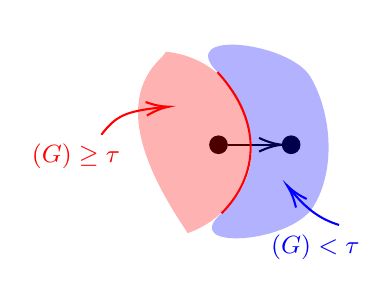
\begin{tikzpicture}[x=0.75pt,y=0.75pt,yscale=-1,xscale=1]
%uncomment if require: \path (0,797); %set diagram left start at 0, and has height of 797

\draw  [draw opacity=0][fill={rgb, 255:red, 0; green, 0; blue, 0 }  ,fill opacity=1 ][line width=0.75]  (496.6,610.1) .. controls (496.6,607.61) and (498.61,605.6) .. (501.1,605.6) .. controls (503.59,605.6) and (505.6,607.61) .. (505.6,610.1) .. controls (505.6,612.59) and (503.59,614.6) .. (501.1,614.6) .. controls (498.61,614.6) and (496.6,612.59) .. (496.6,610.1) -- cycle ;
%Shape: Circle [id:dp40521627665044346] 
\onslide<7->{\draw  [draw opacity=0][fill={rgb, 255:red, 0; green, 0; blue, 0 }  ,fill opacity=1 ][line width=0.75]  (531.6,610.1) .. controls (531.6,607.61) and (533.61,605.6) .. (536.1,605.6) .. controls (538.59,605.6) and (540.6,607.61) .. (540.6,610.1) .. controls (540.6,612.59) and (538.59,614.6) .. (536.1,614.6) .. controls (533.61,614.6) and (531.6,612.59) .. (531.6,610.1) -- cycle ;}
%Straight Lines [id:da7845811693503539] 
\onslide<7->{\draw    (505.6,610.1) -- (529.6,610.1) ;
\draw [shift={(531.6,610.1)}, rotate = 180] [color={rgb, 255:red, 0; green, 0; blue, 0 }  ][line width=0.75]    (10.93,-3.29) .. controls (6.95,-1.4) and (3.31,-0.3) .. (0,0) .. controls (3.31,0.3) and (6.95,1.4) .. (10.93,3.29)   ;}
\onslide<8->{%Shape: Path Data [id:dp33471174830726835] 
\draw  [draw opacity=0][fill={rgb, 255:red, 255; green, 0; blue, 0 }  ,fill opacity=0.3 ] (516.6,610.1) .. controls (516.6,629.85) and (503.88,646.63) .. (486.18,652.69) .. controls (485.73,651.87) and (485.21,651.01) .. (484.6,650.1) .. controls (464.6,620.1) and (452.6,589.1) .. (472.6,569.1) .. controls (474.01,567.69) and (475.06,566.42) .. (475.78,565.29) .. controls (498.67,567.4) and (516.6,586.66) .. (516.6,610.1) -- cycle ;
%Shape: Polygon Curved [id:ds8534078006559433] 
\draw  [draw opacity=0][fill={rgb, 255:red, 0; green, 0; blue, 255 }  ,fill opacity=0.3 ] (500.6,575.1) .. controls (480.07,554.2) and (535.53,560.4) .. (545.53,577.6) .. controls (555.53,594.8) and (557.93,622) .. (546.73,640) .. controls (535.53,658) and (481.93,661.2) .. (502.6,643.1) .. controls (523.27,625) and (521.13,596) .. (500.6,575.1) -- cycle ;
Shape: Circle [id:dp6323258260851117] 
%Curve Lines [id:da49729789960688] 
\draw [color={rgb, 255:red, 255; green, 0; blue, 0 }  ,draw opacity=1 ]   (500.6,575.1) .. controls (522.6,599.1) and (520.6,625.1) .. (502.6,643.1) ;
%Curve Lines [id:da9781828675291866] 
\draw [color={rgb, 255:red, 255; green, 0; blue, 0 }  ,draw opacity=1 ]   (444.67,605.25) .. controls (451.94,596.04) and (455.92,593.88) .. (475.32,591.93) ;
\draw [shift={(477.17,591.75)}, rotate = 174.56] [color={rgb, 255:red, 255; green, 0; blue, 0 }  ,draw opacity=1 ][line width=0.75]    (10.93,-3.29) .. controls (6.95,-1.4) and (3.31,-0.3) .. (0,0) .. controls (3.31,0.3) and (6.95,1.4) .. (10.93,3.29)   ;
%Curve Lines [id:da9665845518826721] 
\draw [color={rgb, 255:red, 0; green, 0; blue, 255 }  ,draw opacity=1 ]   (559.17,648.75) .. controls (549.13,645.63) and (542.82,640.32) .. (535.36,631.22) ;
\draw [shift={(534.17,629.75)}, rotate = 51.34] [color={rgb, 255:red, 0; green, 0; blue, 255 }  ,draw opacity=1 ][line width=0.75]    (10.93,-3.29) .. controls (6.95,-1.4) and (3.31,-0.3) .. (0,0) .. controls (3.31,0.3) and (6.95,1.4) .. (10.93,3.29)   ;

% Text Node
\draw (409.67,608) node [anchor=north west][inner sep=0.75pt]  [font=\small,color={rgb, 255:red, 255; green, 0; blue, 0 }  ,opacity=1 ]  {$\w(G) \geq \tau $};
% Text Node
\draw (525,652) node [anchor=north west][inner sep=0.75pt]  [font=\small,color={rgb, 255:red, 0; green, 0; blue, 255 }  ,opacity=1 ]  {$\w(G) < \tau $};}


\end{tikzpicture}
